%\documentclass[
  bibliography=totoc,     % Literatur im Inhaltsverzeichnis
  captions=tableheading,  % Tabellenüberschriften
  titlepage=firstiscover, % Titelseite ist Deckblatt
]{scrartcl}

% Paket float verbessern
\usepackage{scrhack}

% Warnung, falls nochmal kompiliert werden muss
\usepackage[aux]{rerunfilecheck}

% unverzichtbare Mathe-Befehle
\usepackage{amsmath}
% viele Mathe-Symbole
\usepackage{amssymb}
% Erweiterungen für amsmath
\usepackage{mathtools}

% Fonteinstellungen
\usepackage{fontspec}
% Latin Modern Fonts werden automatisch geladen
% Alternativ zum Beispiel:
%\setromanfont{Libertinus Serif}
%\setsansfont{Libertinus Sans}
%\setmonofont{Libertinus Mono}

% Wenn man andere Schriftarten gesetzt hat,
% sollte man das Seiten-Layout neu berechnen lassen
\recalctypearea{}

% deutsche Spracheinstellungen
\usepackage[ngerman]{babel}


\usepackage[
  math-style=ISO,    % ┐
  bold-style=ISO,    % │
  sans-style=italic, % │ ISO-Standard folgen
  nabla=upright,     % │
  partial=upright,   % │
  mathrm=sym,        % ┘
  warnings-off={           % ┐
    mathtools-colon,       % │ unnötige Warnungen ausschalten
    mathtools-overbracket, % │
  },                       % ┘
]{unicode-math}

% traditionelle Fonts für Mathematik
\setmathfont{Latin Modern Math}
% Alternativ zum Beispiel:
%\setmathfont{Libertinus Math}

\setmathfont{XITS Math}[range={scr, bfscr}]
\setmathfont{XITS Math}[range={cal, bfcal}, StylisticSet=1]

% Zahlen und Einheiten
\usepackage[
  locale=DE,                   % deutsche Einstellungen
  separate-uncertainty=true,   % immer Unsicherheit mit \pm
  per-mode=symbol-or-fraction, % / in inline math, fraction in display math
]{siunitx}

% chemische Formeln
\usepackage[
  version=4,
  math-greek=default, % ┐ mit unicode-math zusammenarbeiten
  text-greek=default, % ┘
]{mhchem}

% richtige Anführungszeichen
\usepackage[autostyle]{csquotes}

% schöne Brüche im Text
\usepackage{xfrac}

% Standardplatzierung für Floats einstellen
\usepackage{float}
\floatplacement{figure}{htbp}
\floatplacement{table}{htbp}

% Floats innerhalb einer Section halten
\usepackage[
  section, % Floats innerhalb der Section halten
  below,   % unterhalb der Section aber auf der selben Seite ist ok
]{placeins}

% Seite drehen für breite Tabellen: landscape Umgebung
\usepackage{pdflscape}

% Captions schöner machen.
\usepackage[
  labelfont=bf,        % Tabelle x: Abbildung y: ist jetzt fett
  font=small,          % Schrift etwas kleiner als Dokument
  width=0.9\textwidth, % maximale Breite einer Caption schmaler
]{caption}
% subfigure, subtable, subref
\usepackage{subcaption}

% Grafiken können eingebunden werden
\usepackage{graphicx}

% schöne Tabellen
\usepackage{tabularray}
\UseTblrLibrary{booktabs, siunitx}

% Verbesserungen am Schriftbild
\usepackage{microtype}

% Literaturverzeichnis
\usepackage[
  backend=biber,
]{biblatex}
% Quellendatenbank
\addbibresource{lit.bib}
\addbibresource{programme.bib}

% Hyperlinks im Dokument
\usepackage[
  german,
  unicode,        % Unicode in PDF-Attributen erlauben
  pdfusetitle,    % Titel, Autoren und Datum als PDF-Attribute
  pdfcreator={},  % ┐ PDF-Attribute säubern
  pdfproducer={}, % ┘
]{hyperref}
% erweiterte Bookmarks im PDF
\usepackage{bookmark}

% Trennung von Wörtern mit Strichen
\usepackage[shortcuts]{extdash}

\author{%
  Vincent Wirsdörfer\\%
  \href{mailto:vincent.wirsdoerfer@udo.edu}{authorA@udo.edu}%
  \and%
  Joris Daus\\%
  \href{mailto:joris.daus@udo.edu}{authorB@udo.edu}%
}
\publishers{TU Dortmund – Fakultät Physik}


%\begin{document}
\section{Versuchsaufbau}
\label{sec:Versuchsaufbau}

Hauptbestandteil des im folgend protokollierten Versuchs ist eine Kupfer-Röntgenröhre, ein LiF-Kristall sowie ein Geiger-Müller Zählrohr. Die wesentlichen 
elektronischen Einstellungen wie zum Beispiel der \emph{Kristallwinkel} oder die \emph{Inegrationszeit} sind im Röntengerät implementiert und lassen 
sich über ein separates Computerprogrammm je nach Versuchsteil optimieren. Die Anordnung und Positionierung der soeben aufgeführten Elemente lässt sich 
anhand der folgenden Abbildung nachvollziehen.

\begin{figure}[H]
    \centering
    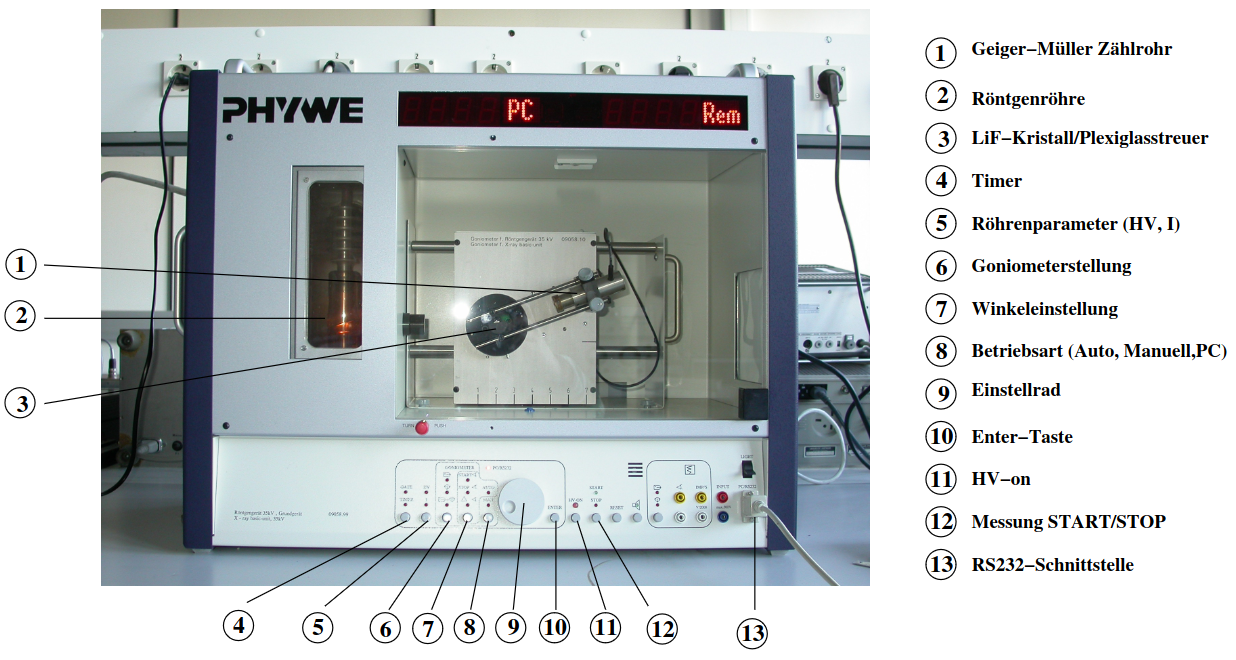
\includegraphics[height=6cm]{content/Aufbau.png}
    \caption{Versuchsanordnung zur Röntgenemission und -absorption\cite{Versuchsanleitung_v602}.}
    \label{fig:Aufbau}
\end{figure}

\noindent Über das Programm \emph{measure} kann die \emph{Messart}, der \emph{Drehmodus}, der anzufahrende \emph{Kristallwinkel} und die \emph{Integrationszeit}
der Messung angepasst werden. Ferner können grundsätzliche Einstellungen wie eine Beschleunigungsspannung von $U_\text{B} = \qty{35}{\kilo\volt}$ und ein Emissionstrom 
von $I = \qty{1}{\milli\ampere}$ überprüft werden. Bevor die erste Messung  gestartet werden kann, wird die Halterung der Blende sowie des LiF-Kristalls kontrolliert. 
Zusätzlich muss die Scheibe des Röntgengeräts geöffnet und fest verschlossen werden, um mit der Aufnahme der Spektren beginnen zu können. 

\section{Versuchsdurchführung}
\label{sec:Versuchsdurchfuehrung}

\subsection{Bragg Bedingung}

Im ersten Teil des Versuchs wird die sog. \emph{Bragg Bedingung} untersucht. Im Programm wird hierzu der LiF-Kristall auf einen \emph{festen Kristallwinkel} von 
$\theta = \qty{14}{\degree}$ gestellt. Das Winkelintervall des Geiger-Müller-Zählrohrs deckt den Bereich von $\alpha_\text{GM} = \qty{26}{\degree}$ bis 
$\alpha_\text{GM} = \qty{30}{degree}$ ab, wobei der Winkelzuwachs $\increment\alpha = \qty{0.1}{\degree}$ beträgt. Die Integrationszeit pro Winkel wird auf einen 
Wert von $\increment{}t = \qty{5}{\sec}$ eingestellt.

\subsection{Emissionsspektrum einer Cu-Röntgenröhre}

Entgegen des vorherigen Versuchsteils wird nun der \emph{2:1 Koppelmodus} aktiviert und das Röntgenspektrum in einem Winkelbereich 
$\qty{4}{\degree} \leq \theta \geq \qty{26}{\degree}$ bei einer Schrittweite von $\increment\alpha = \qty{0.2}{\degree}$ aufgenommen. Die Integrationszeit liegt 
bei $\increment{}t = \qty{5}{\second}$.

\subsection{Das Absorptionsspektrum}

Im letzten Versuchsteil werden die Absorptionsspektren verschiedener Elemente aufgenommen. Dazu werden die zu untersuchenden Proben vor das Geiger-Müller-Zählrohr 
gesetzt und befestigt. Bei den Elementen handelt es sich um Brom, Gallium, Strontiom, Zink und Zirconium. Für alle Proben ist eine Integrationszeit von 
$\increment{}t = \qty{20}{\sec}$ und eine Schrittweite von \qty{0.1}{\degree} zu wählen. Das Messintervall umfasst den Bereich von $\pm\qty{1}{\degree}$ um 
den Bragg-Winkel. Da dieser Winkel für jedes Elemente echt verschieden ist, muss der Messbereich kontinuierlich angepasst werden. Die Bragg-Winkel der jeweiligen 
Elemente lauten folgendermaßen:

\begin{align*}
    \theta_\text{Br} &= \qty{13.2}{\degree} \\
    \theta_\text{Ga} &= \qty{17.3}{\degree} \\  
    \theta_\text{Sr} &= \qty{11.1}{\degree} \\  
    \theta_\text{Zn} &= \qty{18.7}{\degree} \\  
    \theta_\text{Zr} &= \qty{9.9}{\degree} \\  
\end{align*}

\section{Messwerte}
\label{sec:Messwerte}

Die gemessenen Wertepaare {$2\theta_\text{i}, N_\text{i}$}, wobei $N_\text{i}$ die gemessen Zählraten beschrieibt, zur Überprüfung der Bragg Bedingung werden in der 
folgenden Tabelle dargestellt.

\begin{table}[H]
    \centering
    \caption{Messdaten zur Überprüfung der Bragg-Bedingung.}
    \label{tab:BraggBedingungTab}
    \sisetup{table-format=2.1}
    \begin{tblr}{
        colspec = {S S},
        row{1} = {guard, mode=math},
    }
    \toprule
    2\theta \mathbin{/} \unit{\degree} & N \\
    \midrule
    26.0  &  12.0  \\
    26.2  &  16.0  \\
    26.4  &  24.0  \\
    26.6  &  35.0  \\
    26.8  &  46.0  \\
    27.0  &  58.0  \\
    27.2  &  65.0  \\
    27.4  &  74.0  \\
    27.6  &  85.0  \\
    27.8  &  85.0  \\
    28.0  &  77.0  \\
    28.2  &  77.0  \\
    28.4  &  61.0  \\
    28.6  &  55.0  \\
    28.8  &  41.0  \\
    29.0  &  35.0  \\
    29.2  &  26.0  \\
    29.4  &  18.0  \\
    29.6  &  8.0   \\
    29.8  &  14.0  \\
    30.0  &  7.0   \\
    \bottomrule
    \end{tblr}
\end{table}

\noindent Im Folgenden wird der aufgenommene Datensatz des Emissionsspektrums der Cu-Röntgenröhre aufgelistet.

\begin{table}[H]
    \caption{Messdaten des Cu-Emissionsspektrums.}
    \label{tab:Wellenlaenge}
    \sisetup{table-format=2.1}
    \begin{minipage}[t]{0.5\textwidth}
        \vspace{0pt}
        \centering
    \begin{tblr}{
        colspec = {S S},
        row{1} = {guard, mode = math},
        }
        \toprule
        2\theta \mathbin{/} \unit{\degree} & N \\
        \midrule
            8.0	  &  13.0 \\
            8.3	  &  11.0 \\
            8.8	  &  12.0 \\
            9.2	  &  11.0 \\
            9.6	  &  11.0 \\
            10.0  &	 17.0 \\
            10.4  &	 31.0 \\
            10.8  &	 39.0 \\
            11.2  &	 49.0 \\
            11.6  &	 55.0 \\
            12.0  &	 54.0 \\
            12.4  &	 56.0 \\
            12.8  &	 65.0 \\
            13.2  &	 69.0 \\
            13.6  &	 69.0 \\
            14.0  &	 77.0 \\
            14.4  &	 73.0 \\
            14.8  &	 77.0 \\
            15.2  &	 73.0 \\
            15.6  &	 79.0 \\
            16.0  &	 76.0 \\
            16.4  &	 80.0 \\
            16.7  &	 82.0 \\
            17.2  &	 80.0 \\
            17.6  &	 85.0 \\
            18.0  &	 81.0 \\
            18.4  &	 82.0 \\
            18.7  &	 85.0 \\
            19.2  &	 91.0 \\
            19.6  &	 83.0 \\
            20.0  &	 83.0 \\
            20.4  &	 94.0 \\
            20.7  &	 87.0 \\
    \end{tblr}
\end{minipage} \hfill
\begin{minipage}[t]{0.5\textwidth}
        \vspace{0pt}
        \centering
    \begin{tblr}{
            colspec={S S},
            row{1} = {guard, mode = math},
        }
        \toprule
        2\theta \mathbin{/} \unit{\degree} & N \\
        \midrule
            21.2  &  93.0 \\
            21.6  &  97.0 \\
            22.0  &  86.0 \\
            22.4  &  94.0 \\
            22.7  &  91.0 \\
            23.2  &  92.0 \\
            23.6  &  95.0 \\
            24.0  &  89.0 \\
            24.4  &  92.0 \\
            24.8  &  95.0 \\
            25.2  &  97.0 \\
            25.6  &  95.0 \\
            26.0  &  95.0 \\
            26.4  &  79.0 \\
            26.8  &  76.0 \\
            27.2  &  85.0 \\
            27.6  &  76.0 \\
            28.0  &  81.0 \\
            28.4  &  75.0 \\
            28.8  &  0.0  \\
            29.2  &  78.0 \\
            29.6  &  81.0 \\
            30.0  &  72.0 \\
            30.4  &  77.0 \\
            30.8  &  74.0 \\
            31.2  &  68.0 \\
            31.6  &  69.0 \\
            32.0  &  67.0 \\
            32.4  &  64.0 \\
            32.8  &  69.0 \\
            33.2  &  62.0 \\
            33.5  &  61.0 \\
            34.0  &  58.0 \\     
        \end{tblr}
    \end{minipage}\hfill
\end{table}

\begin{table}[H]
    \caption{Messdaten des Cu-Emissionsspektrums.}
    \label{tab:Wellenlaenge}
    \sisetup{table-format=2.1}
    \begin{minipage}[t]{0.5\textwidth}
        \vspace{0pt}
        \centering
    \begin{tblr}{
        colspec = {S S},
        row{1} = {guard, mode = math},
        }
        \toprule
        2\theta \mathbin{/} \unit{\degree} & N \\
        \midrule
            34.4  &  68.0  \\ 
            34.8  &  59.0  \\ 
            35.2  &  60.0  \\  
            35.5  &  52.0  \\  
            36.0  &  57.0  \\  
            36.4  &  56.0  \\  
            36.8  &  54.0  \\  
            37.2  &  47.0  \\  
            37.5  &  44.0  \\   
            38.0  &  48.0  \\  
            38.4  &  49.0  \\   
            38.8  &  45.0  \\   
            39.2  &  51.0  \\   
            39.5  &  106.0 \\
            40.0  &  565.0 \\
            40.4  &  638.0 \\
            40.8  &  89.0  \\
            41.2  &  78.0  \\
            41.5  &  65.0  \\
            42.0  &  56.0  \\
            42.4  &  56.0  \\
            42.8  &  54.0  \\
    \end{tblr}
\end{minipage} \hfill
\begin{minipage}[t]{0.5\textwidth}
        \vspace{0pt}
        \centering
    \begin{tblr}{
            colspec={S S},
            row{1} = {guard, mode = math},
        }
        \toprule
        2\theta \mathbin{/} \unit{\degree} & N \\
        \midrule
            43.2  &  66.0   \\
            43.5  &  67.0   \\ 
            44.0  &  125.0  \\ 
            44.4  &  1719.0 \\
            44.8  &  2215.0 \\
            45.2  &  1239.0 \\
            45.5  &  79.0   \\
            46.0  &  53.0   \\
            46.4  &  41.0   \\
            46.8  &  43.0   \\
            47.2  &  36.0   \\
            47.5  &  35.0   \\
            48.0  &  32.0   \\
            48.4  &  32.0   \\
            48.8  &  31.0   \\
            49.2  &  30.0   \\ 
            49.6  &  24.0   \\ 
            50.0  &  25.0   \\ 
            50.4  &  28.0   \\ 
            50.8  &  23.0   \\ 
            51.2  &  25.0   \\
            51.6  &  20.0   \\ 
            52.0  &  22.0   \\
        \end{tblr}
    \end{minipage}\hfill
\end{table}

\noindent Abschließend werden die Tabellen abgebildet, welche die Datensätze der Absorptionsspektren beinahlten.

\begin{table}[H]
    \label{tab:Wellenlaenge}
    \sisetup{table-format=2.1}
    \begin{minipage}[t]{0.5\textwidth}
        \vspace{0pt}
        \centering
        \caption{Absorptionsspektrum von Brom.}
    \begin{tblr}{
        colspec = {S S},
        row{1} = {guard, mode = math},
        }
        \toprule
        2\theta \mathbin{/} \unit{\degree} & N \\
        \midrule
            24.4  &  6.0  \\ 
            24.8  &  5.0  \\   
            25.2  &  4.0  \\  
            25.6  &  6.0  \\  
            26.0  &  8.0  \\ 
            26.4  &  11.0 \\
            26.8  &  13.0 \\
            27.2  &  11.0 \\
            27.6  &  10.0 \\
            28.0  &  11.0 \\
            28.4  &  10.0 \\
    \end{tblr}
\end{minipage} \hfill
\begin{minipage}[t]{0.5\textwidth}
        \vspace{0pt}
        \centering
        \caption{Absorptionsspektrum von Gallium.}
    \begin{tblr}{
            colspec={S S},
            row{1} = {guard, mode = math},
        }
        \toprule
        2\theta \mathbin{/} \unit{\degree} & N \\
        \midrule
            32.5  &  12.0 \\
            33.0  &  12.0 \\
            33.4  &  11.0 \\
            33.8  &  12.0 \\
            34.2  &  19.0 \\
            34.5  &  25.0 \\
            35.0  &  29.0 \\
            35.4  &  27.0 \\
            35.8  &  25.0 \\
            36.2  &  24.0 \\
            36.5  &  22.0 \\      
        \end{tblr}
    \end{minipage}\hfill
\end{table}

\begin{table}[H]
    \label{tab:Wellenlaenge}
    \sisetup{table-format=2.1}
    \begin{minipage}[t]{0.5\textwidth}
        \vspace{0pt}
        \centering
        \caption{Absorptionsspektrum von Strontiom.}
    \begin{tblr}{
        colspec = {S S},
        row{1} = {guard, mode = math},
        }
        \toprule
        2\theta \mathbin{/} \unit{\degree} & N \\
        \midrule
            20.2  &  12.0 \\
            20.6  &  14.0 \\
            21.0  &  11.0 \\
            21.4  &  17.0 \\
            21.7  &  27.0 \\
            22.2  &  38.0 \\
            22.6  &  42.0 \\
            23.0  &  40.0 \\
            23.4  &  37.0 \\
            23.8  &  35.0 \\
            24.2  &  34.0 \\
    \end{tblr}
\end{minipage} \hfill
\begin{minipage}[t]{0.5\textwidth}
        \vspace{0pt}
        \centering
        \caption{Absorptionsspektrum von Zink.}
    \begin{tblr}{
            colspec={S S},
            row{1} = {guard, mode = math},
        }
        \toprule
        2\theta \mathbin{/} \unit{\degree} & N \\
        \midrule
            35.4  &	 17.0 \\
            35.8  &	 17.0 \\
            36.2  &	 15.0 \\
            36.5  &	 17.0 \\
            37.0  &	 27.0 \\
            37.4  &	 32.0 \\
            37.8  &	 32.0 \\
            38.2  &	 29.0 \\
            38.5  &	 30.0 \\
            39.0  &	 31.0 \\
            39.4  &	 44.0 \\   
        \end{tblr}
    \end{minipage}\hfill
\end{table}

\begin{table}[H]
    \centering
    \caption{Emissionsspektrum von Zirconium.}
    \label{tab:BraggBedingungTab}
    \sisetup{table-format=2.1}
    \begin{tblr}{
        colspec = {S S},
        row{1} = {guard, mode=math},
    }
    \toprule
    2\theta \mathbin{/} \unit{\degree} & N \\
    \midrule
        17.7  &  30.0 \\
        18.2  &  29.0 \\
        18.6  &  29.0 \\
        19.0  &  29.0 \\
        19.4  &  34.0 \\
        19.7  &  45.0 \\
        20.2  &  52.0 \\
        20.6  &  52.0 \\
        21.0  &  55.0 \\
        21.4  &  51.0 \\
        21.7  &  52.0 \\
    \bottomrule
    \end{tblr}
\end{table}

%\end{document}

